\chapter[BOOM: Declarative Scheduling]{BOOM: Declarative Scheduling}
\label{ch:boom}

The Berkeley Orders Of Magnitude (BOOM) project began with an experiment in
construction, by implementing a substantial piece of distributed software in a
data-centric, declarative style.  Upon review of recent literature on
data center infrastructure (e.g.,~\cite{chubby,gfs-sosp,dynamo,mapreduce-osdi}),
we observed that most of the complexity in these systems relates to the
management of various forms of asynchronously-updated state, including
sessions, protocols and storage.  Although quite complex, few of these systems
involve intricate, uninterrupted sequences of computational steps.  Hence, we
suspected that data center infrastructure might be a good initial litmus test
for our hypotheses about building distributed software.

\emph{\BOOMA} is an API-compliant reimplementation of the HDFS distributed file
system and the Hadoop MapReduce engine~\cite{boom}.  These two components were
named \emph{\BOOM-FS} and \emph{\BOOM-MR}, respectively.  In writing \BOOMA, we
preserved the Java API ``skin'' of HDFS and Hadoop, but replaced complex
internal state with a set of relations, and replaced key system logic with code
written in a declarative language.  In this chapter, we focus on our
implementation of \BOOM-MR, but provide some experimental evaluations of
\BOOM-FS.

The remainder of this chapter is organized as follows.
Section~\ref{ch:boom:sec:jol} describes a new Java-based \OVERLOG library that
we used execute \OVERLOG programs within the (Java-based) Hadoop
infrastructure.  Section~\ref{ch:boom:sec:port} presents BOOM-MR as a
declarative MapReduce scheduler, and describes how we embedded it into the
Hadoop system by replacing the existing scheduling code written in Java with
\OVERLOG.  Section~\ref{ch:boom:sec:eval} evaluates the resulting declarative
scheduler against the original unmodified Hadoop scheduler by comparing the
response times of jobs scheduled by both.  Finally,
Section~\ref{ch:boom:sec:relwork} examines some of the related work and
Section~\ref{ch:boom:sec:conclusion} provides a chapter summary.

\section{Java \OVERLOG Library (JOL)}
\label{ch:boom:sec:jol}

P2's lack of support for stratified Datalog forced us to implement a number of
imperative hacks that often involved (event) manipulations of the underlying
dataflow fixpoints.  Most of these hacks were required for detecting the
termination of a group of rules, which would have been implicitly handled by
imposing a natural stratum boundary (e.g., count aggregate).  Our workaround
involved adding a number of conditions that detected the stratum boundary, and
ensuring that these ``conditions'' were computed in separate P2 dataflow
fixpoints.  This was a hard lesson, which led us to develop an entirely new
\OVERLOG implementation that supports stratified Datalog.  We present this new
system, called \JOL, here.

Like P2, \JOL compiles \OVERLOG programs into pipelined dataflow graphs of
operators (similar to ``elements'' in the Click modular router~\cite{click}).
\JOL provides \emph{metaprogramming} support akin to P2's Evita Raced
extension (Chapter~\ref{ch:evita}): each \OVERLOG program is compiled into a
representation that is captured in rows of tables.  Program testing,
optimization and rewriting can be written concisely as metaprograms in \OVERLOG
that manipulate those tables.

The original \OVERLOG implementation ({\em P2}) is aging, and lacked support
for Java, so we developed a new Java-based \OVERLOG runtime we call {\em \JOL.}
We originally developed \JOL as a Datalog (only) library for the Pig
system~\cite{pig-sigmod}.  The idea was for \JOL, along with the Evita Raced
extensions, to be the rule-based optimizer for the PigLatin language.  This
initial version of \JOL was used to perform a number of heuristic~\footnote{Pig
had no support for statistics at the time.} rewrites for PigLatin queries, and
it can be applied to Pig through a patch~\cite{jira-360}.

The \JOL system matured when we targeted the Hadoop stack, which required tight
integration between \OVERLOG and Java code.  The latest version of \JOL
includes Java-based extensibility in the model of Postgres~\cite{postgres}.  It
supports Java classes as abstract data types, allowing Java objects to be
stored in fields of tuples, and Java methods to be invoked on those fields from
\OVERLOG.  \JOL also allows Java-based aggregation functions to run on sets of
column values, and supports Java \emph{table functions}: Java iterators
producing tuples, which can be referenced in \OVERLOG rules as ordinary
relations.  We made significant use of each of these features in \BOOMA.

%In addition, inspired by the ideas of Evita Raced, we metaprogrammed \JOL's
%core execution loop and scheduler in \OVERLOG as well.  Rather than using a
%traditional event loop, in \JOL all inbound events (i.e., tuples) are passed
%into a single dataflow compiled from the system's runtime metaprogram.  This
%dataflow ``routes'' tuples to appropriate branches corresponding to different
%rules, using a scheduler specified in \OVERLOG.  Space prevents a thorough
%discussion of this design, but we mention it here because of our experience
%modifying the runtime rules as described in Section~\ref{sec:perf}.

\section{\BOOM-MR: A Declarative MapReduce Scheduler}
\label{ch:boom:sec:port}

In this section, we describe our declarative version of the Hadoop MapReduce
scheduled, which we call \BOOM-MR.  We used \BOOM-MR to explore embedding a
data-centric rewrite of a non-trivial component into an existing procedural
system.  MapReduce scheduling policies are one issue that has been treated in
recent literature (e.g.,~\cite{zaharia-late,delay-sched}).  To enable credible
work on MapReduce scheduling, we wanted to remain true to the basic structure
of the Hadoop MapReduce codebase, so we proceeded by understanding that code,
mapping its core state into a relational representation, and then writing
\OVERLOG rules to manage that state in the face of new messages delivered by
the existing Java APIs.  

Section~\ref{ch:boom:sec:hadoop} provides quick review of the Hadoop MapReduce
scheduler component.  In Section~\ref{ch:boom:sec:tables} we capture the
entities and relationships of the Hadoop scheduler in four table catalog.
Using these tables, we develop a scheduling policy in
Section~\ref{ch:boom:sec:scheduler} that models the FIFO policy in stock
Hadoop, but using fewer lines of code.  We then add to it, in
Section~\ref{ch:boom:sec:late}, the LATE policy scheduling ``speculative''
tasks.  Our declarative LATE port took {\em orders of magnitude} less time and
code, compared to the Java port~\cite{jira-2141}, once the basic relational
infrastructure was in place.

\subsection{Hadoop MapReduce Scheduler}
\label{ch:boom:sec:hadoop}

Recall in Hadoop MapReduce, there is a single master node called the \emph{\JT}
which manages a number of worker nodes called \emph{{\TT}s}.  A job is divided
into a set of map and reduce \emph{tasks}.  The {\JT} assigns tasks to worker
nodes.  Each map task reads an input chunk from the distributed file system,
runs a user-defined map function, and partitions output key/value pairs into
hash buckets on the local disk.  Reduce tasks are created for each hash bucket.
Each reduce task fetches the corresponding hash buckets from all mappers, sorts
locally by key, runs a user-defined reduce function and writes the results to
the distributed file system.

Each {\TT} has a fixed number of slots for executing tasks (two maps and two
reduces by default).  A heartbeat protocol between each {\TT} and the {\JT} is
used to update the {\JT}'s bookkeeping of the state of running tasks, and drive
the scheduling of new tasks: if the {\JT} identifies free {\TT} slots, it will
schedule further tasks on the {\TT}.  Also, Hadoop will attempt to schedule
\emph{speculative} tasks to reduce a job's response time if it detects
``straggler'' nodes~\cite{mapreduce-osdi}.

\subsection{Table-izing MapReduce}
\label{ch:boom:sec:tables}

Our initial goal was to port the Hadoop \JT code to \OVERLOG.  We began by
identifying the key state maintained by the {\JT}.  This state includes both
data structures to track the ongoing status of the system and transient state
in the form of messages sent and received by the {\JT}.  We captured this
information the four \OVERLOG tables shown in Table~\ref{ch:boom:tbl:hcatalog}.

\begin{table}
\ssp
\centering
\begin{tabular}{|l|l|l|} \hline
\textit{Name}   & \textit{Description} & \textit{Relevant attributes} \\ \hline\hline
job         & Job definitions   & \underline{JobId}, Priority, SubmitTime, Status, JobConf \\ \hline
task         & Task definitions  & \underline{JobId}, \underline{TaskId}, Type, Partition, Status \\ \hline
taskAttempt  & Task attempts      & \underline{JobId}, \underline{TaskId}, \underline{AttemptId}, Progress, \\
             &       & State, Phase, Tracker, InputLoc, Start, Finish \\ \hline
taskTracker  & {\TT} State  & \underline{Name}, Hostname, State, \\
             &       & MapCount, ReduceCount, MaxMap, MaxReduce\\ \hline
\end{tabular}
\caption{\BOOM-MR relations defining {\JT} state.}
\label{ch:boom:tbl:hcatalog}
\end{table}

The \ol{job} relation contains a single row for each job submitted to the
{\JT}. In addition to some basic metadata, each job tuple contains an attribute
called $JobConf$ that holds a Java object constructed by legacy Hadoop
code, which captures the configuration of the job. The \ol{task} relation
identifies each task within a job. The attributes of this relation identify the
task type (map or reduce), the input ``partition'' (a chunk for map tasks, a
bucket for reduce tasks), and the current running status.

A task may be attempted more than once, due to speculation or if the initial
execution attempt failed.  The \ol{taskAttempt} relation maintains the state
of each such attempt.  In addition to a progress percentage and a state
(running/completed), reduce tasks can be in any of three phases: copy, sort, or
reduce. The $Tracker$ attribute identifies the {\TT} that is assigned to
execute the task attempt. Map tasks also need to record the location of their
input data, which is given by $InputLoc$. 

The \ol{taskTracker} relation identifies each {\TT} in the cluster with a
unique name.  The hostname, current running state, and task workload of the \TT
are also part of this relation.  The $MapCount$ and $ReduceCount$ attributes
indicate how many map and reduce tasks are currently running on the \TT.  The
maximum number of map and reduce tasks that the \TT is able to support are
given by the $MaxMap$ and $MaxReduce$ attributes; this is in keeping with
Hadoop which specifies these values in each message from a \TT to the \JT.

\OVERLOG rules are used to update the {\JT}'s tables by converting inbound messages
into \ol{job}, \ol{taskAttempt} and \ol{taskTracker} tuples. These rules
are mostly straightforward. Scheduling decisions are encoded in the
\ol{taskAttempt} table, which assigns tasks to {\TT}s. A scheduling policy is
simply a set of rules that join against the \ol{taskTracker} relation to find
\TT{}s with unassigned slots, and schedules tasks by inserting tuples into
\ol{taskAttempt}. This architecture makes it easy for new scheduling policies
to be defined.

\subsection{MapReduce Scheduling in \OVERLOG}
\label{ch:boom:sec:scheduler}

MapReduce scheduling has been the subject of recent research, and one of our
early motivations for building \BOOMA was to make this research extremely easy
to carry out.  In our initial \BOOM-MR prototype, we implemented Hadoop's
default First-Come-First-Served (or FIFO) policy for task scheduling, which was
captured in 9 rules (96 lines) of scheduler policy.  Next, we implemented the
recently-proposed LATE policy~\cite{zaharia-late} to evaluate both (a) the
difficulty of prototyping a new policy, and (b) the faithfulness of our
\OVERLOG-based execution to that of Hadoop using two separate scheduling
algorithms.

\subsubsection{First-Come-First-Served Scheduling}

\begin{figure}
\label{fig:joborder}
\ssp
\centering
\begin{boxedminipage}{\linewidth}
\ol{s1} {\bf minPriority}(min$<$Priority$>$) :- \\
\datalogspace {\bf job}(JobId, Priority, Status, SubmitTime, ...), \\
\datalogspace {\bf task}(JobId, TaskId, Type, \_, \_, StartTime, ...), \\
\datalogspace $StartTime < 0$; \\
	
\ol{s2} {\bf minPriorityStartTime}(Priority, min$<$SubmitTime$>$) :- \\
\datalogspace {\bf job}(JobId, Priority, Status, SubmitTime, ...), \\
\datalogspace {\bf task}(JobId, TaskId, Type, \_, \_, StartTime, ...), \\
\datalogspace $StartTime < 0$; \\

\ol{s3} {\bf highestPriorityJob}(JobId) :- \\
\datalogspace {\bf minPriority}(Priority), \\
\datalogspace {\bf minPriorityStartTime}(Priority, StartTime), \\
\datalogspace {\bf job}(JobId, Priority, Status, SubmitTime, ...); \\
\end{boxedminipage}
\caption{\label{ch:boom:fig:joborder}The highest priority job that still has unscheduled tasks ($StartTime < 0$).}
\end{figure}

In this section, we outline the declarative specification for Hadoop's default
task scheduling policy.  The policy schedules tasks from the job with the
highest priority.  A job's scheduling order is defined by its $Priority$
followed by its $SubmitTime$ attributes.  The tasks from the job that is first
in the scheduling order are scheduled before any other tasks from other jobs.

Figure~\ref{ch:boom:fig:joborder} captures this constraint in three rules, which
identify the job whose tasks are considered first when \TT slots are available.
Rule \ol{s1} identifies the job with the minimum priority, while rule~\ol{s2}
determines, for each priority, the job with the earliest submit time.  Both
\ol{s1} and \ol{s2} only consider jobs that have unscheduled tasks, which are
identified by a negative $StartTime$ value in the \ol{task} relation.  Rule
\ol{s3} joins the result of rules \ol{s1} and \ol{s2} to identify the overall
highest priority job with unscheduled tasks.

Scheduling individual tasks from the highest priority job occurs when a \TT
performs a heartbeat exchange with the \JT and has some number of available map
or reduce task slots.  A all tasks are scheduled based solely on slot
availability; if a task slot is available then schedule a task from the job
with the highest priority.  To avoid data movement costs, the default policy
will consider the location of the input to the map task and try to schedule the
map task close to a machine that hosts its input data.  During a heartbeat
exchange with a \TT that has available map slots, the \JT will schedule map
tasks from the highest priority job whose input data resides closest to the
\TT.  Ideally, the input to the map task resides on the same machine or rack
but if not then an arbitrary map task is scheduled, without considering other
queued jobs.

\begin{figure}
\ssp
\centering
\begin{boxedminipage}{\linewidth}
s4 {\bf mapTaskLocality}(TaskId, Tracker, Locality) :- \\
\datalogspace {\bf heartbeat}(Tracker, TrackerStatus, MapSlots, ReduceSlots), \\
\datalogspace {\bf hightestPriorityJob}(JobId), \\
\datalogspace {\bf task}(JobId, TaskId, Type, \_, InputSplits, StartTime, \_), \\
\datalogspace $StartTime < 0$, $Type == "map"$, \\
\datalogspace \{ \\
\datalogspace \datalogspace {\bf if} (InputSplits.contains(TrackerStatus.getHost())) \{ \\
\datalogspace \datalogspace \datalogspace Locality := 1; // same machine \\
\datalogspace \datalogspace \} {\bf else if} (InputSplits.contains(TrackerStatus.getRack()) \{ \\
\datalogspace \datalogspace \datalogspace Locality := 2; // same rack \\
\datalogspace \datalogspace \} {\bf else} \{ \\
\datalogspace \datalogspace \datalogspace Locality := 3;  \\
\datalogspace \datalogspace \} \\
\datalogspace \}; \\
	
s5 {\bf schedule}(Tracker, bottomK$<$MapID, MapSlots$>$) :- \\
\datalogspace {\bf mapTaskLocality}(TaskId, Tracker, Locality), \\
\datalogspace {\bf heartbeat}(Tracker, TrackerStatus, MapSlots, ReduceSlots), \\
\datalogspace $MapSlots > 0$, \\
\datalogspace MapID := new OrderedMapID(TaskId, Locality); \\

\end{boxedminipage}
\caption{\label{ch:boom:fig:schedule} Map task locality priority scheduler.}
\end{figure}

Figure~\ref{ch:boom:fig:schedule} shows two rules that together implement this
default Hadoop policy, which schedules map tasks near the data.  When a \TT
heartbeat is received, rule \ol{s4} assigns a locality metric to unscheduled
tasks that belong to the highest priority job.  \JOL supports the ability to
add Java code at the end of a rule body, delineated within brackets \{ ...  \}.
This Java code executes last in the rule body, and will only see those tuples
that represent actual deductions.  In rule \ol{s4}, the bracketed Java code
assigns a Locality metric according to the proximity of the heartbeat \TT to
the map input data.

The result of rule \ol{s4} is evaluated in rule \ol{s5}, which schedules the
map tasks whose inputs reside closest to the heartbeat \TT.  The {\bf bottomK}
aggregate orders the $MapID$s from lowest to highest $Locality$ and chooses the
lowest map tasks in this order, not exceeding the number of available map slots
($MapSlots$).  Each result tuple from rule \ol{s5} is converted, through a few
imperative steps in the Java language, into a schedule action message that is
returned to the \TT in its RPC call to the \JT.  The reduce task scheduling
rule simply schedules reduces tasks from the highest priority job based on the
reduce slot capacity of the heartbeat \TT, as per stock Hadoop.

\subsection{Task Speculation in \OVERLOG}
\label{ch:boom:sec:late}

\begin{figure}[p]
\ssp
\begin{boxedminipage}{\linewidth}

// Compute progress rate per task \\
\ol{l1} {\bf taskPR}(JobId, TaskId, Type, ProgressRate) :- \\
\datalogspace {\bf task}(JobId, TaskId, Type, \_, \_, \_, Status), \\
\datalogspace $Status.state() != FAILED$,  \\
\datalogspace Time := $Status.finish() > 0$ ? Status.finish() : currentTimeMillis(), \\
\datalogspace ProgressRate := Status.progress() / (Time - Status.start()); \\

// For each job, compute 25th pctile rate across tasks \\
\ol{l2} {\bf slowTaskThreshold}(JobId, Type, percentile$<$0.25, PRate$>$) :- \\
\datalogspace {\bf taskPR}(JobId, TaskId, Type, PRate); \\

// Compute progress rate per tracker \\
\ol{l3} {\bf trackerPR}(Tracker, JobId, Type, avg$<$PRate$>$) :- \\ 
\datalogspace {\bf task}(JobId, TaskId, Type, \_), \\
\datalogspace {\bf taskAttempt}(JobId, TaskId, \_, Progress, State, Phase, Tracker, Start, Finish), \\
\datalogspace $State != FAILED$, \\
\datalogspace Time := $Finish > 0$ ? Finish : currentTimeMillis(), \\ 
\datalogspace PRate := Progress / (Time - Start);  \\

// For each job, compute 25th pctile rate across trackers \\
\ol{l4} {\bf slowNodeThreshold}(JobId, Type, percentile<0.25, AvgPRate>) :- \\
\datalogspace {\bf trackerPR}(\_, JobId, Type, AvgPRate); \\

// Compute available map/reduce slots \\
\ol{l5} {\bf speculativeCap}(sum<MapSlots>, sum<ReduceSlots>) :- \\
\datalogspace {\bf taskTracker}( ... MapCount, ReduceCount, MaxMap, MaxReduce), \\
\datalogspace MapSlots := 0.1 * (MaxMap - MapCount), \\
\datalogspace ReduceSlots := 0.1 * (MaxReduce - ReduceCount); \\
\end{boxedminipage}
\caption{\OVERLOG to compute statistics for LATE.}
\label{fig:latePolicy}
\end{figure}

With the basic scheduling logic behind us, we turn now to the topic of
scheduling speculative tasks.  The LATE policy presents a scheme for scheduling
speculative tasks based on {\em straggler} tasks~\cite{zaharia-late}.  There
are two aspects to each policy: choosing which tasks to speculatively
re-execute, and choosing {\TT}s to run those tasks.  Original Hadoop
re-executes a task if its progress is more than 0.2 (on a scale of $[0..1]$)
below the mean progress of similar tasks; it assigns speculative tasks using
the same policy as it uses for initial tasks.  LATE chooses tasks to re-execute
via an {\em estimated finish time} metric based on the task's \emph{progress
rate}.  Moreover, it avoids assigning speculative tasks to {\TT}s that exhibit
slow performance executing similar tasks, in hopes of preventing the creation
of new stragglers.

The LATE policy is specified in the paper via just three lines of pseudocode,
which make use of three performance statistics called $SlowNodeThreshold$,
$SlowTaskThreshold$ and $SpeculativeCap$.  The first two of these statistics
correspond to the $25^{th}$ percentiles of progress rates across {\TT}s and
across tasks, respectively.  The $SpeculativeCap$ indicates the maximum number
of speculative tasks allowed at any given time, which is suggested to be set at
$10\%$ of the total available task slots~\cite{zaharia-late}.

We compute these thresholds via the five \OVERLOG rules shown in
Figure~\ref{fig:latePolicy}.  A task is only considered for speculation if its
progress rate falls below the $SlowTaskThreshold$ in its given category: job
identifier ($JobID$) and task type ($Type$).  Queries \ol{l1} and \ol{l2}
maintain this threshold value for each category.  Query \ol{l1} determines the
progress rate for a given task based on its current progress and running time.
Query \ol{l2} computes the $SlowTaskThreshold$, for each category, by
determining the lower $25^{th}$ percentile of the progress rates.

The LATE policy ensures that speculative tasks execute on ``fast'' nodes by
pruning \TT nodes whose rate of progress for a given task category fall below
some threshold.  Queries \ol{l3} and \ol{l4} maintain this threshold value for
each category.  The first query \ol{l3}, computes the average progress that a
given \TT has made for each task category and stores that result in the
\ol{trackerPR} table.  Query \ol{l4} computes the $SlowNodeThreshold$ for each
category by determining the 25th percentile for each category of progress rates
stored in the \ol{trackerPR} table.  Finally, query \ol{l5} counts the number
of slots that can be used for task speculation.  Integrating the rules into
\BOOM-MR required modifying two additional \OVERLOG rules that identify tasks
to speculatively re-execute, and choose {\TT}s for scheduling those tasks, all
while obeying the SpeculativeCap value.

\section{Evaluation}
\label{ch:boom:sec:eval}

We now validate our declarative specification of both Hadoop's default
First-Come-First-Serve (FCFS) policy and the LATE policy proposed by Zaharia et
al.~\cite{zaharia-late}. Our goals were both to evaluate the difficulty of
building a new policy, and to confirm the faithfulness of our \OVERLOG-based
{\JT} to the Hadoop {\JT} using two different scheduling algorithms.

Implementing the default FCFS policy required 9 rules (96 lines of
code). Implementing the LATE policy required 5 additional \OVERLOG rules (30
lines of code). In comparison, LATE is specified in Zaharia et al.'s paper via
just three lines of pseudocode, but their implementation of the policy for
vanilla Hadoop required adding or modifying over $800$ lines of Java spread 
across $18$ Java class files --- an order of magnitude more than our \OVERLOG implementation. 

We used a 101-node cluster on Amazon EC2. One node executed the Hadoop \JT\ 
and the HDFS \NN, while the remaining 100 nodes served as slaves for running the 
Hadoop {\TT}s and HDFS {\DN}s. Each {\TT} was configured to support executing up 
to two map tasks and two reduce tasks simultaneously. The master node ran on a 
``high-CPU extra large'' EC2 instance with 7.2 GB of memory and 8 virtual cores. 
Our slave nodes executed on ``high-CPU medium'' EC2 instances with 1.7 GB of 
memory and 2 virtual cores. Each virtual core is the equivalent of a 2007-era 2.5Ghz Intel Xeon
processor.


\subsection{First-Come-First-Serve policy}

\begin{figure*}
\ssp
\centering
	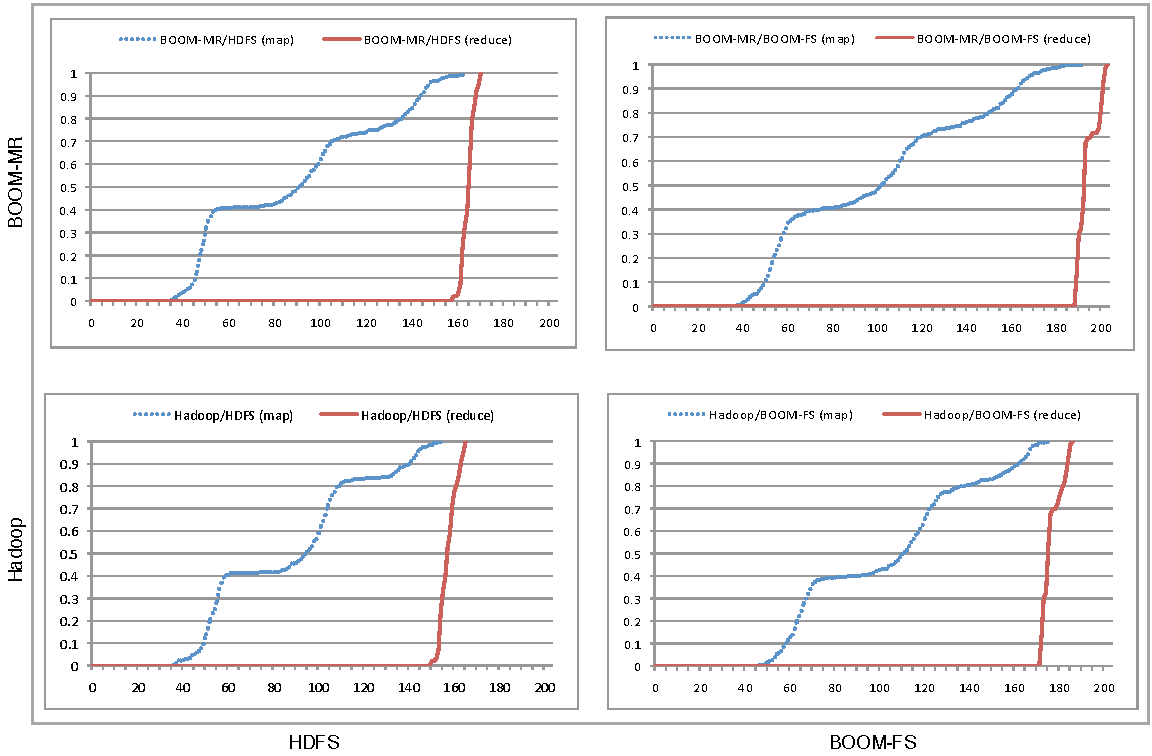
\includegraphics[scale=0.75]{figures/fourgraphs}
\caption{CDFs representing the elapsed time between job startup and task
  completion for both map and reduce tasks, for all combinations of Hadoop and \BOOM-MR
  over HDFS and \BOOM-FS\@.  In each graph, the horizontal axis is
  elapsed time in seconds, and the vertical represents the percentage of tasks completed.}
\label{fig:ec2experiment}
\end{figure*}

While improved performance was not a goal of our work, we wanted to
ensure that the performance of \BOOMA was competitive with Hadoop.
The workload was a wordcount job on a 30 GB file, using 481 map tasks 
and 100 reduce tasks.

Figure~\ref{fig:ec2experiment} contains four graphs comparing the performance of
different combinations of Hadoop MapReduce, HDFS, \BOOM-MR, and \BOOM-FS\@. Each
graph reports a cumulative distribution of the elapsed time in seconds from job
startup to map or reduce task completion. The map tasks complete in three
distinct ``waves.'' This is because only 2 $\times$ 100 map tasks can be
scheduled at once. Although all 100 reduce tasks can be scheduled immediately,
no reduce task can finish until all maps have been completed because each reduce
task requires the output of all map tasks.

The lower-left graph describes the performance of Hadoop running on top of HDFS,
and hence serves as a baseline for the subsequent graphs. The upper-left graph
details \BOOM-MR running over HDFS\@. This graph shows that map and reduce task
durations under \BOOM-MR are nearly identical to Hadoop 18.1. The lower-right
and upper-right graphs detail the performance of Hadoop MapReduce and \BOOM-MR
running on top of \BOOM-FS, respectively. \BOOM-FS performance is slightly
slower than HDFS, but remains competitive.


\subsection{LATE policy}

We now compare the behavior of our LATE implementation with the results observed
by Zaharia et al.\ using Hadoop MapReduce. LATE focuses on how to improve job completion time by reducing the impact of
``straggler'' tasks. To simulate stragglers, we artificially placed additional
load on six nodes. We ran a wordcount job on 30 GB of data, using 481 map tasks
and 400 reduce tasks (which produced two distinct ``waves'' of reduces). We ran
each experiment five times, and report the average over all
runs. Figure~\ref{fig:ec2reduce} shows the reduce task duration CDF for three
different configurations. The plot labeled ``No Stragglers'' represents normal
load, while the ``Stragglers'' and ``Stragglers (LATE)'' plots describe
performance in the presence in stragglers using the default FCFS policy and the
LATE policy, respectively. We omit map task durations, because adding artificial
load had little effect on map task execution --- it just resulted in slightly
slower growth from just below 100\% to completion.

\begin{figure*}
\ssp
  \centering
  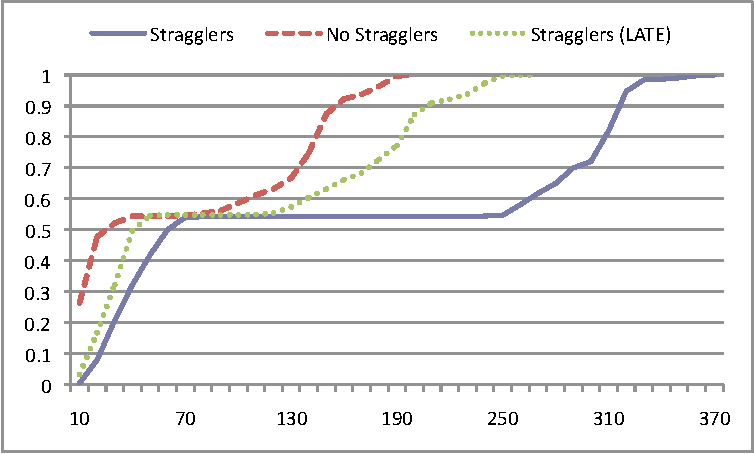
\includegraphics[scale=0.75]{figures/reduce_stragglers}
  \caption{CDF of reduce task duration (secs), with and without stragglers.}
  \label{fig:ec2reduce}
\end{figure*}

The first wave of 200 reduce tasks was scheduled at the beginning of the
job. This first wave of reduce tasks cannot finish until all map tasks have
completed, which increased the duration, hence the large runtime durations indicated in the right
portion of the graph. The second wave of 200 reduce tasks did not experience
delay due to unfinished map work since it was scheduled after all map tasks had
finished. These shorter task durations are reported in the left portion of the
graph. Furthermore, stragglers had less impact on the second wave of reduce
tasks since less work (i.e., no map work) is being performed. Figure~\ref{fig:ec2reduce} 
shows this effect, and also demonstrates how the LATE implementation in {\BOOMA} 
handles stragglers much more effectively than the FCFS policy ported from Hadoop.  
This echoes the results of Zaharia et al.~\cite{zaharia-late}

\section{Related Work}
\label{ch:boom:sec:relwork}

Declarative and data-centric languages have traditionally been considered useful
in very few domains, but things have changed substantially in recent years.
MapReduce~\cite{mapreduce-osdi} has popularized functional dataflow programming
with new audiences in computing.  Also, a surprising breadth of recent research
projects have proposed and prototyped declarative languages, including overlay
networks~\cite{p2:sosp}, three-tier web services~\cite{hilda}, natural language
processing~\cite{dyna}, modular robotics~\cite{meld}, video games~\cite{cornellgames}, 
file system metadata analysis~\cite{wiscfsck}, and compiler analysis~\cite{bddbddb}.

Most of the languages cited above are declarative in the same sense as SQL: they are 
based in first-order logic. Some --- notably MapReduce, but also SGL~\cite{cornellgames} --- are
algebraic or dataflow languages, used to describe the composition of operators that produce and 
consume sets or streams of data.  Although arguably imperative, they are far closer to logic languages 
than to traditional imperative languages like Java or C, and are often amenable to set-oriented optimization 
techniques developed for declarative languages~\cite{cornellgames}. Declarative and dataflow languages 
can also share the same runtime, as demonstrated by recent integrations of MapReduce and SQL
in Hive~\cite{hive-vldb}, DryadLINQ~\cite{DryadLINQ}, HadoopDB~\cite{hadoopdb}, and products from vendors 
such as Greenplum and Aster.

Concurrent with our work, the Erlang language was used to implement a simple MapReduce framework called 
Disco~\cite{disco} and a transactional DHT called Scalaris with Paxos support~\cite{scalaris}. Philosophically, Erlang 
revolves around concurrent {\em actors}, rather than data. A closer comparison of actor-oriented and data-centric design 
styles is beyond the scope of this dissertation, but an interesting topic for future work.

\section{Summary}
\label{ch:boom:sec:conclusion}

The initial version of \BOOM-MR required one person-month of development time.
We spent an additional two person-months debugging and tuning \BOOM-MR's
performance for large jobs.  At the present time, \BOOM-MR represents the
declarative specification of the core task scheduler (9 rules), the speculative
task scheduler (5 rules), recovery from failed tasks (3 rules), and maintaining
various job and task statistics (5 rules).  In total, \BOOM-MR consists of 22
\OVERLOG rules in 156 lines of code, and 1269 lines of Java.  \BOOM-MR is based
on Hadoop version 18.1; we estimate that we removed 6,573 lines from Hadoop
(out of 88,864).  The removed code contained the core scheduling logic and the
data structures that represent the components listed in
Table~\ref{ch:boom:tbl:hcatalog}.  The \OVERLOG patch that replaces the
original Hadoop scheduler contains an order of magnitude fewer lines of code.
The performance of \BOOM-MR is very similar to that of Hadoop MapReduce, as we
discuss in Section~\ref{ch:boom:sec:eval}.

For this ``porting'' exercise, it was handy to leverage \JOL's Java interfaces
and draw the Java/\OVERLOG boundaries flexibly.  This allowed us to focus on
porting the more interesting Hadoop logic into \OVERLOG, while avoiding ports of
relatively mechanical details.  For example, we chose to leave the data
representation of the \emph{jobConf} as a Java object rather than flatten it
into a relation because it had no effect on the scheduling logic.

We found that scheduling policies were a good fit for a declarative language
like \OVERLOG. In retrospect, this is because scheduling can be decomposed into
two tasks: \emph{monitoring} the state of a system and applying \emph{policies}
for how to react to changes to that state. Monitoring is well-handled by \OVERLOG: 
we found that the statistics about {\TT} state required by the LATE policy are naturally 
realized as aggregate functions, and \JOL took care of automatically updating those statistics 
as new messages from {\TT}s arrived. In the next chapter, we will look at importing statistics
taken from the output of a MapReduce job that is continuously monitoring machine and process level statistics.
Once these near real-time monitoring statistics have been imported into \JOL, we can build some 
very interesting scheduling policies around them.

It is also unsurprisingly that a logic language should be well-suited to specifying policy. Indeed, 
the rules in Chapters~\ref{ch:p2} and~\ref{ch:evita} can be viewed as search policies for shortest 
paths in a network and an optimal plan for a query. Moreover, the rules that govern bottom-up
and top-down plan enumeration can be viewed as {\em search strategy} policies. In the current context, we found 
the \BOOM-MR scheduler much simpler to extend and modify than the original Hadoop Java code, as demonstrated 
by our experience with LATE\@.  Informally, the \OVERLOG code in \BOOM-MR seems about as complex as it should be: 
Hadoop's MapReduce task coordination logic is a simple and clean design, and the compactness of \BOOM-MR reflects 
that simplicity appropriately. In Chapter~\ref{ch:hop}, we extended the MapReduce batch-oriented model to a pipelining 
model. Pipelining MapReduce requires operators be coscheduled; a policy that is easily handled by a few extra \OVERLOG 
rules beyond those discussed here.





